\documentclass{article}
\usepackage[utf8]{inputenc}

\title{Ph21 Project 1: Stings and Webs}
\author{Kalliopi Somis }
\date{Winter 2020}

\usepackage{natbib}
\usepackage{graphicx}

\begin{document}

\maketitle

\section{Part 1}
In this project we extract data from the CRTS data set using the python module urllib. For  part 1 we access the HTML page source and use string manipulations to isolate the data. 

\begin{figure}[ht!]
\centering
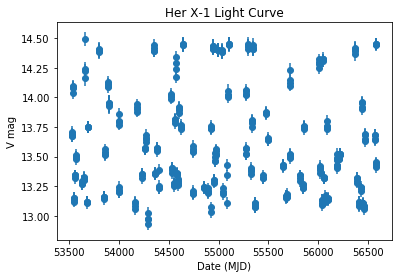
\includegraphics[scale=.7]{lc1.png}
\caption{This light curve of the source Her X-1 plots magnitude vs time. This data was collected from the HTML output. The information was extracted from a python array. The array consisted of tuples of the form [x,y,yerror]. We can set parameters for each point by calling the nth element in each tuple and plot the results using matplotlib}
\label{fig: HTML Light Curve}
\end{figure}

\section{Part 2}
For part 2 we extract the same data set in VOTable format. The VOTable files can be read and manipulated using astropy. We can then use 'get first table' to retrieve the data instead of searching for it and using string manipulations. 

\begin{figure}[ht!]
\centering
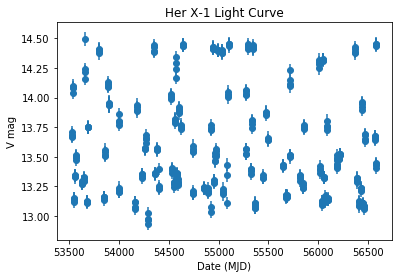
\includegraphics[scale=.7]{lc2.png}
\caption{This light curve of the source Her X-1 plots magnitude vs time. as you can see it lools the same as Figure 1, but this data was extracted from a a VOTable file. The table can be called directly and each column of data has a key.  we assign the key ObsTime to x, Mag to y and Magerr to yerror and plot the results using matplotlib}
\label{fig: VOTable Light Curve}
\end{figure}

\end{document}
